% ----------------------------------------------------------
% VALIDAÇÕES DE SEGURANÇA, INTERFACE E CÓDIGO
% ----------------------------------------------------------
\section{Validações de segurança, interface e código}
Nessa seção serão abordados algumas validações que fizemos na nossa aplicação e a justificativa deles.

\subsection{Teste dos \emph{headers} da API}
Para os testes de \emph{headers} de segurança, usamos o site \gls{secheaders}, onde pudemos ver em qual nota se enquadrava nossa \ac{api}. Testamos um dos nossos \emph{endpoints} (O resultado é o mesmo para todos), e durante o primeiro teste, o site nos deu nota F, pela resposta da nossa aplicação não conter nenhum \emph{header} de segurança, então com base nesse resultado, adicionamos essas dependências que faltavam e conseguimos subir a nota, como demonstra a \autoref{sec-headers}.

\begin{figure}[H]
	\centering
	\caption{\label{sec-headers}Validação dos \emph{headers}}
	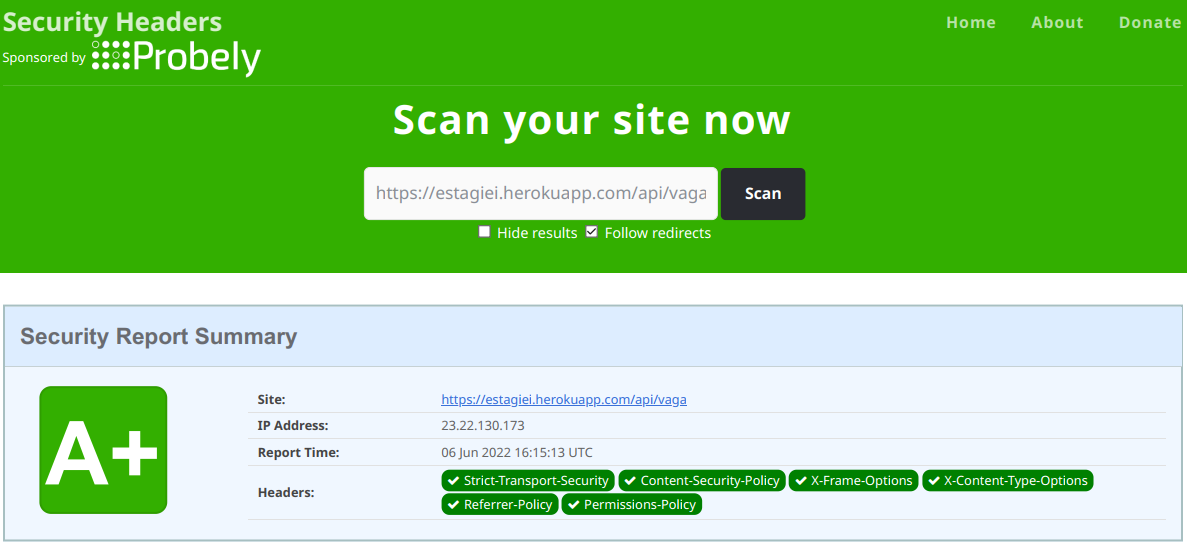
\includegraphics[width=0.95\textwidth]{../imagens/web-tests/grade-security-headers.png}
	\fonte{\cite{securityheaders}}
\end{figure}

\begin{figure}[htb]
	\caption{\label{qr-url-swagger}URL da documentação dos nossos endpoints (Swagger UI)}
	\begin{center}
		\geraQRCode{https://estagiei.herokuapp.com/api/swagger-ui/}
		\legend{\url{https://estagiei.herokuapp.com/api/swagger-ui/}}
		\fonte{Os Autores.}
	\end{center}
\end{figure}

\subsection{Teste de \ac{tls} do \gls{frontend}}
Também testamos nosso \emph{website} com relação ao certificado \ac{tls}, que indica se um site utiliza o protocolo \ac{https} ou não. E por nossa aplicação estar hospedada no \gls{netlify}, ele automaticamente já providencia um certificado com o \gls{letsencrypt} quando criamos um domínio personalizado. Assim como mostra a \autoref{grade-server-test}, nossa aplicação possui um certificado \ac{tls} ativo.

\begin{figure}[H]
	\centering
	\caption{\label{grade-server-test}Teste de \ac{tls}}
	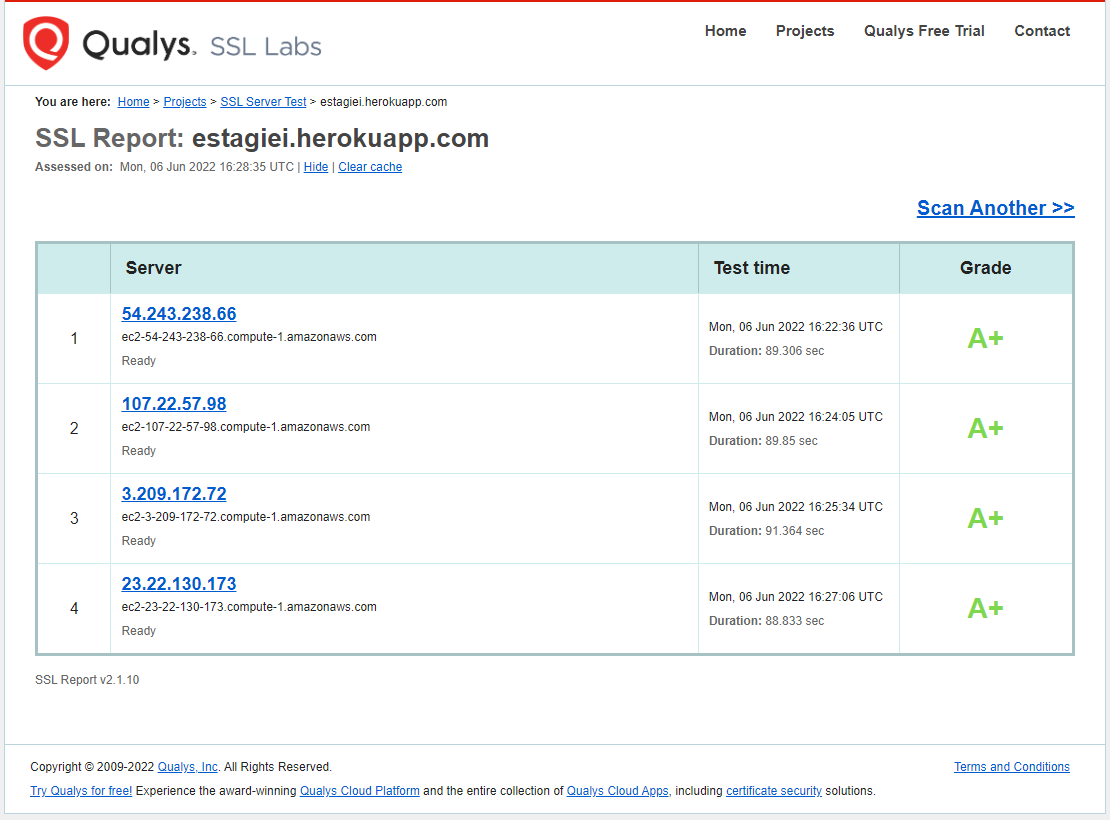
\includegraphics[width=0.95\textwidth]{../imagens/web-tests/grade-server-test.png}
	\fonte{\cite{ssllabs}}
\end{figure}

\begin{figure}[htb]
	\caption{\label{qr-url-frontend}URL do \gls{frontend} da nossa aplicação}
	\begin{center}
		\geraQRCode{https://estagiei.netlify.app/}
		\legend{\url{https://estagiei.netlify.app/}}
		\fonte{Os Autores.}
	\end{center}
\end{figure}

\subsection{Teste de desempenho do \gls{frontend}}
Através da extensão \gls{lighthouse}, verificamos como estava o desempenho, acessibilidade, etc. Da nossa tela de login, e percebemos pontos a serem melhorados, principalmente na questão do desempenho. Pontos esses que serão ajustados no próximo semestre. A \autoref{lighthouse-test} ilustra o resultado.

\begin{figure}[H]
	\centering
	\caption{\label{lighthouse-test}Teste de desempenho do \gls{frontend}}
	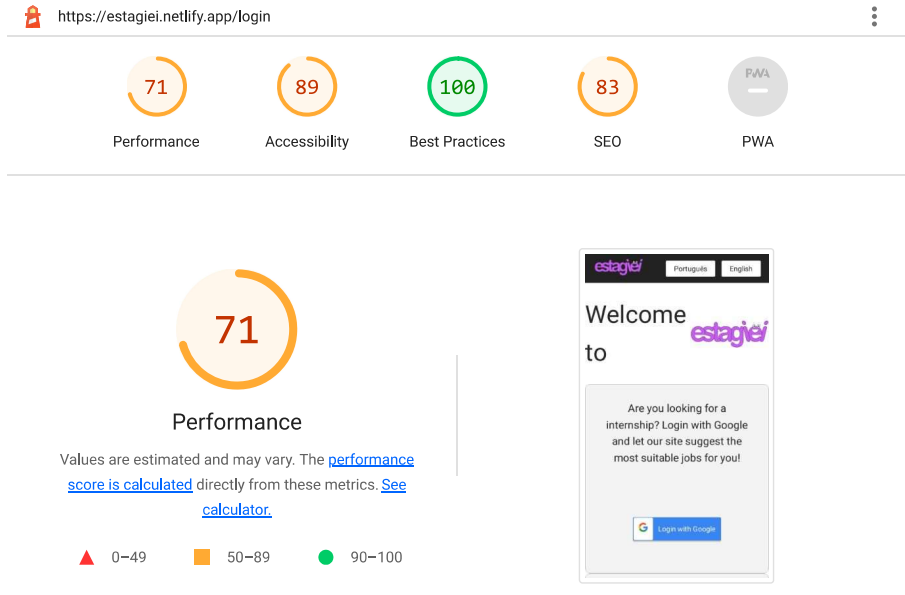
\includegraphics[width=0.95\textwidth]{../imagens/web-tests/lighthouse-test.png}
	\fonte{\gls{lighthouse}}
\end{figure}

\subsection{Análise de código}
Fizemos também uma verificação no nosso código, tanto no \gls{frontend} como no \gls{backend}, e o resultado foi relativamente satisfatório, faltando apenas alguns pontos que serão melhorados ao longo do tempo. As figuras \autoref{better-code-front} e \autoref{better-code-back} demonstram os resultados do \gls{frontend} e \gls{backend} respectivamente.

\begin{figure}[H]
	\centering
	\caption{\label{better-code-front}Análise de código do \gls{frontend}}
	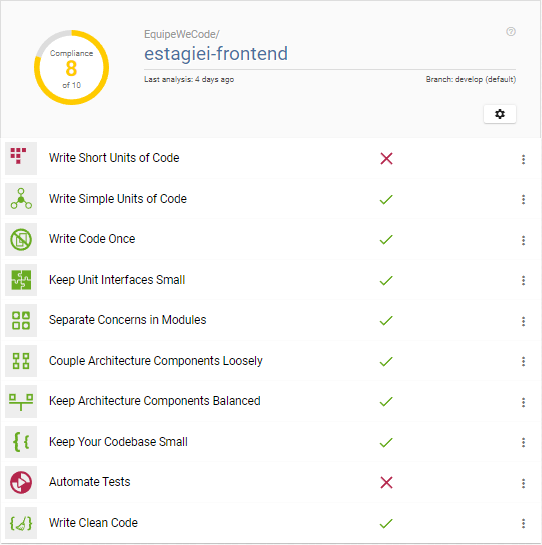
\includegraphics[width=0.95\textwidth]{../imagens/web-tests/better-code-front.png}
	\fonte{\gls{bettercode}}
\end{figure}

\begin{figure}[H]
	\centering
	\caption{\label{better-code-back}Análise de código do \gls{backend}}
	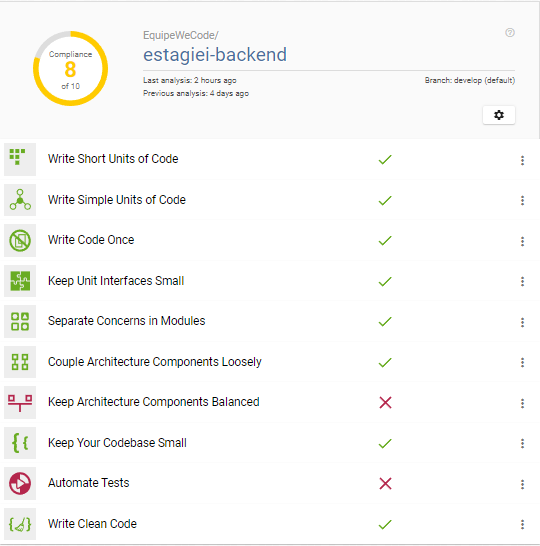
\includegraphics[width=0.95\textwidth]{../imagens/web-tests/better-code-back.png}
	\fonte{\gls{bettercode}}
\end{figure}

\subsection{Validador \ac{html}}
Fizemos também uma verificação no nosso \ac{html} do \ac{frontend}. A \autoref{validador-html} demonstra o resultado.

\begin{figure}[H]
	\centering
	\caption{\label{validador-html}Validação do \ac{html}}
	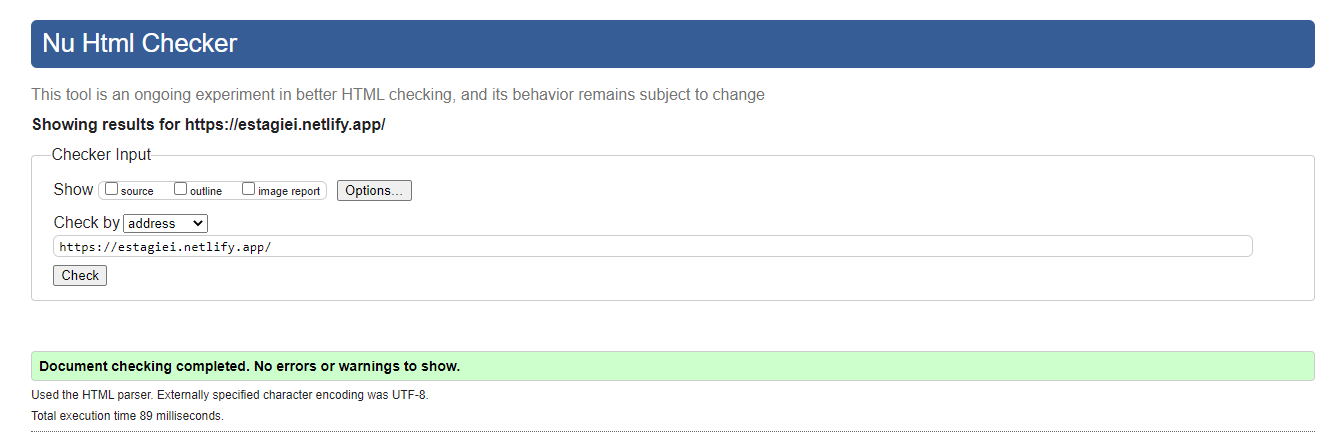
\includegraphics[width=0.95\textwidth]{../imagens/web-tests/validador-html.png}
	\fonte{\cite{w3c-validator}}
\end{figure}

